%!TEX program = xelatex
%!TEX options=--shell-escape
\documentclass[12pt]{article}

%
\usepackage[scheme=plain]{ctex}
%
\usepackage{fontspec}
%
\usepackage[margin = 1in]{geometry}

%
\usepackage[dvipsnames]{xcolor}
\usepackage[many]{tcolorbox}

%
\usepackage{amsmath}
\usepackage{amssymb}
\usepackage{amsthm}
%
\usepackage{tensor}
%
\usepackage{slashed}
\usepackage{physics}
\usepackage{simpler-wick}

%
\usepackage{mathtools}

%
\usepackage{bm}
\newcommand{\dbar}{\dif\hspace*{-0.18em}\bar{}\hspace*{0.2em}}
\DeclareMathAlphabet\mathbfcal{OMS}{cmsy}{b}{n}
%\usepackage{bbold}
\newcommand*{\dif}{\mathop{}\!\mathrm{d}}
\newcommand*{\euler}{\mathrm{e}}
\newcommand*{\imagi}{\mathrm{i}}

\renewcommand{\vec}[1]{\boldsymbol{\mathbf{#1}}}

\usepackage{caption}
\usepackage{multirow}
\usepackage{enumitem}

%
\usepackage{mathrsfs}
\usepackage{dsfont}

%
\usepackage{hyperref}
\hypersetup{
    colorlinks=true,
    linkcolor=violet,
    filecolor=blue,
    urlcolor=blue,
    citecolor=cyan,
}

%
\usepackage{graphicx}
\usepackage{subfig}
%
\graphicspath{{../figures/}}

\usepackage{tikz}
\usetikzlibrary{positioning}
\usetikzlibrary{calc}

\usepackage{listings}
\usepackage{lstautogobble}
\lstset{
    basicstyle=\ttfamily,
    columns=fullflexible,
    autogobble=true,
}

%
\usepackage{indentfirst}
%
\setlength{\parindent}{2em}
\linespread{1.25}

%
% \setmainfont{Times New Roman}

\title{Note}
\author{Feng-Yang Hsieh}
\date{}

\begin{document}
\maketitle

\section{Higgs Production}% (fold)
\label{sec:higgs_production}
    We want to apply deep learning methods to distinguish vector boson fusion (VBF) from gluon-gluon fusion (GGF) and Higgs production at the LHC.

    We want to apply the CWoLa method, then can use the real data without knowing the true label.
% section higgs_production (end)
\section{Sample Preparation}% (fold)
\label{sec:sample_preparation}
    \subsection{Monte Carlo samples}% (fold)
    \label{sub:monte_carlo_samples}
        We consider Standard Model (SM) di-photon Higgs events produced via GGF and VBF channels at a center-of-mass energy of $\sqrt{s} = 14$ TeV. The Higgs boson events are generated using \verb|MadGraph 3.3.1|~\cite{Alwall:2014hca} for both GGF and VBF production. The Higgs decays into the di-photon final state, and the parton showering and hadronization are simulated using \verb|Pythia 8.306|~\cite{Sjostrand:2014zea}. The detector simulation is conducted by \verb|Delphes 3.4.2|~\cite{deFavereau:2013fsa}. Jet reconstruction is performed using \verb|FastJet 3.3.2|~\cite{Cacciari:2011ma} with the anti-$k_t$ algorithm~\cite{Cacciari:2008gp} and a jet radius of $R = 0.4$. These jets are required to have transverse momentum $p_{\text{T}} > 25$ GeV.

        The following \verb|MadGraph| scripts generate Monte Carlo samples for each production channel.
        \paragraph{GGF Higgs Sample Generation}
        \begin{lstlisting}
            generate p p > h QCD<=99 [QCD]
            output GGF_Higgs
            launch GGF_Higgs

            shower=Pythia8
            detector=Delphes
            analysis=OFF
            madspin=OFF
            done

            set run_card nevents 100000
            set run_card ebeam1 7000.0
            set run_card ebeam2 7000.0

            set run_card use_syst False

            set pythia8_card 25:onMode = off
            set pythia8_card 25:onIfMatch = 22 22
            done
        \end{lstlisting}
        \paragraph{VBF Higgs Sample Generation}
        \begin{lstlisting}
            define v = w+ w- z
            generate p p > h j j $$v
            output VBF_Higgs
            launch VBF_Higgs

            shower=Pythia8
            detector=Delphes
            analysis=OFF
            madspin=OFF
            done

            set run_card nevents 100000
            set run_card ebeam1 7000.0
            set run_card ebeam2 7000.0

            set run_card use_syst False

            set pythia8_card 25:onMode = off
            set pythia8_card 25:onIfMatch = 22 22
            done
        \end{lstlisting}
    % subsection monte_carlo_samples (end)
    \subsection{Event selection}% (fold)
    \label{sub:event_selection}
        The selection cuts after the \verb|Delphes| simulation:
        \begin{itemize}
            \item $n_{\gamma}$ cut: The number of photons should be at least 2.
            \item $n_{j}$ cut: The number of jets should be at least 2.
            \item $m_{\gamma\gamma}$ cut: The invariant mass of two leading photons $m_{\gamma\gamma}$ are required $\text{120 GeV} \le m_{\gamma\gamma} \le \text{130 GeV}$.
        \end{itemize}

        Table~\ref{tab:GGF_VBF_Higgs_cutflow_number} summarizes the cutflow number at different selection cuts.
        \begin{table}[htpb]
            \centering
            \caption{Number of passing events and passing rates for GGF and VBF Higgs production at different selection cuts.}
            \label{tab:GGF_VBF_Higgs_cutflow_number}
            \begin{tabular}{l|rr|rr}
                Cut                    & GGF    & pass rate & VBF    & pass rate \\ \hline
                Total                  & 100000 & 1         & 100000 & 1         \\
                $n_{\gamma}$ cut       & 48286  & 0.48      & 53087  & 0.53      \\
                $n_j$ cut              & 9302   & 0.09      & 42860  & 0.43      \\
                $m_{\gamma\gamma}$ cut & 8864   & 0.09      & 40694  & 0.41     
            \end{tabular}
        \end{table}
        
        Figure~\ref{fig:mjj_deta_distribution} shows the distributions of $m_{jj}$ (the invariant mass of the two leading jets) and $\Delta\eta_{jj}$ (the pseudorapidity difference between the two leading jets). The scatter plot of $m_{jj}$ versus $\Delta\eta_{jj}$ is presented in Figure~\ref{fig:mjj_deta_scatter}.
        \begin{figure}[htpb]
            \centering
            \subfloat[$m_{jj}$ distribution]{
                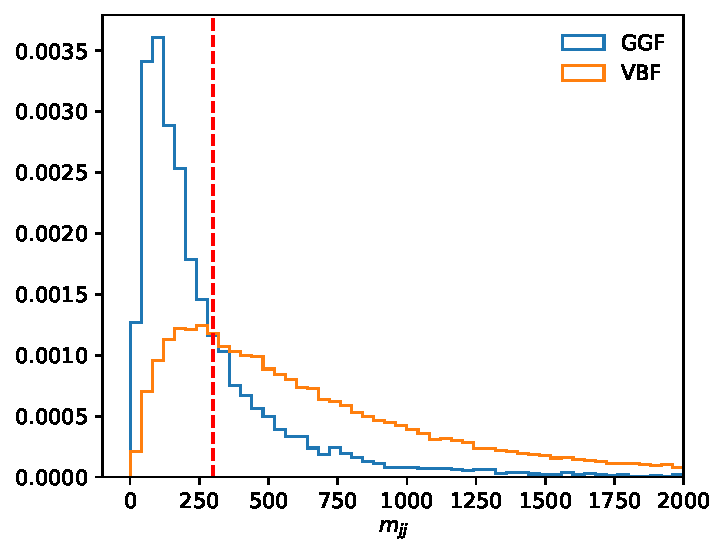
\includegraphics[width=0.45\textwidth]{mjj_distribution.pdf}
            }
            \subfloat[$\Delta\eta_{jj}$ distribution]{
                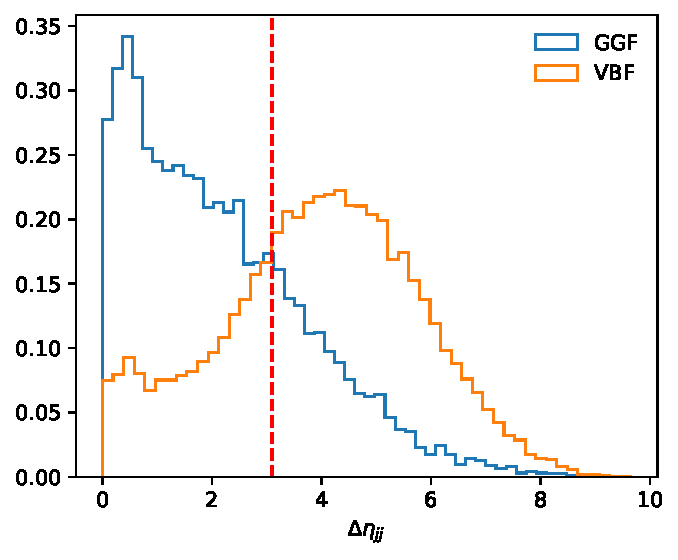
\includegraphics[width=0.45\textwidth]{deta_distribution.pdf}
            }
            \caption{Distributions of the invariant mass $m_{jj}$ and pseudorapidity difference $\Delta\eta_{jj}$ of the two leading jets. Red dashed lines are selection cuts used to construct mixed datasets.}
            \label{fig:mjj_deta_distribution}
        \end{figure}
        \begin{figure}[htpb]
            \centering
            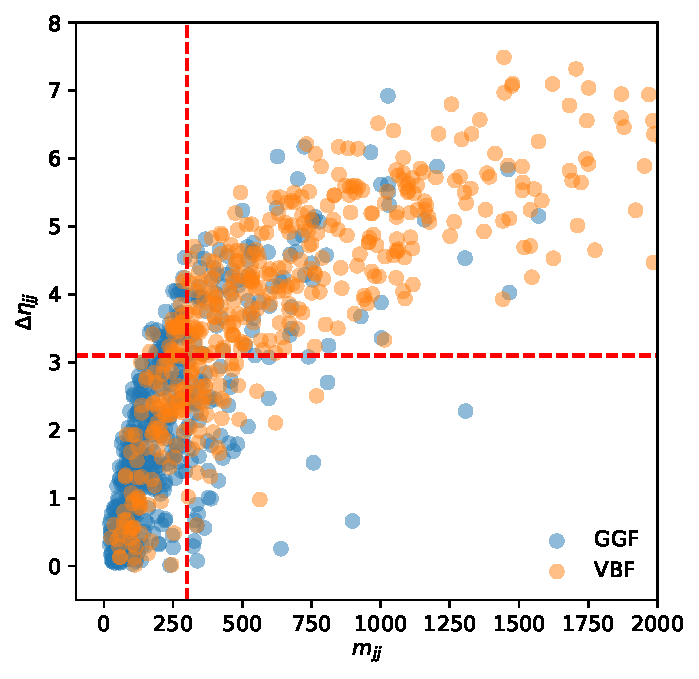
\includegraphics[width=0.45\textwidth]{mjj_deta_scatter_plot.pdf}
            \caption{Scatter plot of $m_{jj}$ versus $\Delta\eta_{jj}$. Red dashed lines are selection cuts used to construct mixed datasets.}
            \label{fig:mjj_deta_scatter}
        \end{figure}
    % subsection event_selection (end)
    \subsection{Event image}% (fold)
    \label{sub:event_image}
        The inputs for the neural networks are event images~\cite{Kasieczka:2019dbj,deOliveira:2015xxd, Kasieczka2017nv}. These images are constructed from events that pass the kinematic selection criteria described in section~\ref{sub:event_selection}. Each event image has three channels corresponding to calorimeter towers, tracks, and photons. The following preprocessing steps are applied to all event constituents:
        \begin{enumerate}
            \item Translation: Compute the $p_{\text{T}}$-weighted center in the $\phi$ coordinates, then shift this point to the origin.
            \item Flipping: Flip the highest $p_{\text{T}}$ quadrant to the first quadrant.
            \item Pixelation: Pixelate in a $\eta \in [-5, 5],\ \phi \in [-\pi, \pi]$ box, with $40 \times 40$ pixels 
        \end{enumerate}

        Figure~\ref{fig:GGF_VEF_event_image} shows the event images for GGF and VBF production modes.
        \begin{figure}[htpb]
            \centering
            \subfloat[GGF: Calorimeter Tower]{
                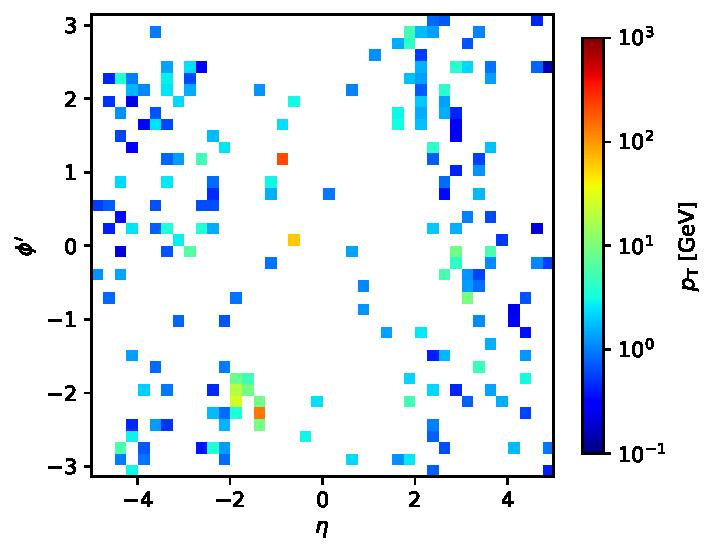
\includegraphics[width=0.45\textwidth]{event_image_GGF-tower.pdf}
            }
            \subfloat[VBF: Calorimeter Tower]{
                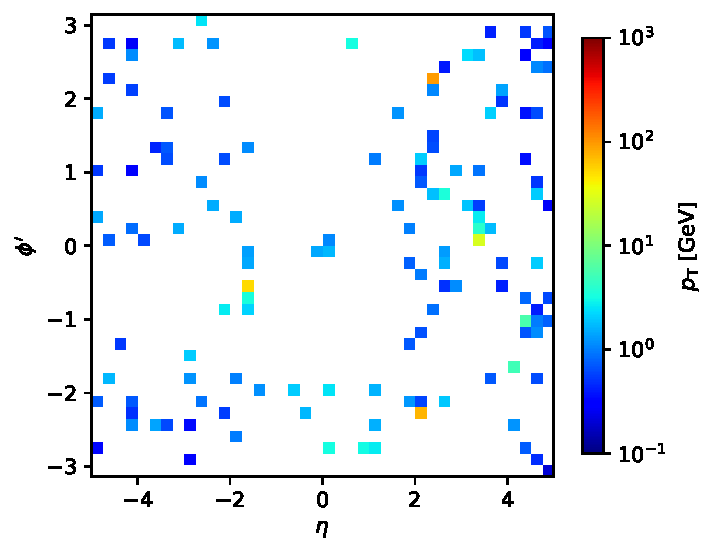
\includegraphics[width=0.45\textwidth]{event_image_VBF-tower.pdf}
            } \\
            \subfloat[GGF: Track]{
                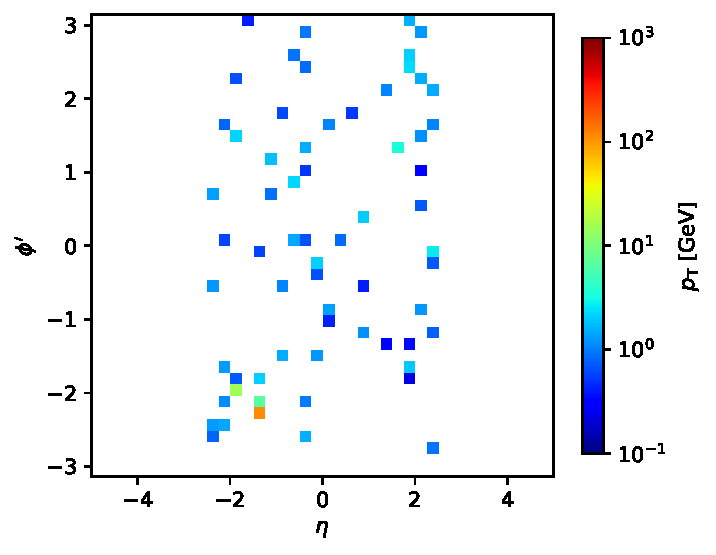
\includegraphics[width=0.45\textwidth]{event_image_GGF-track.pdf}
            }
            \subfloat[VBF: Track]{
                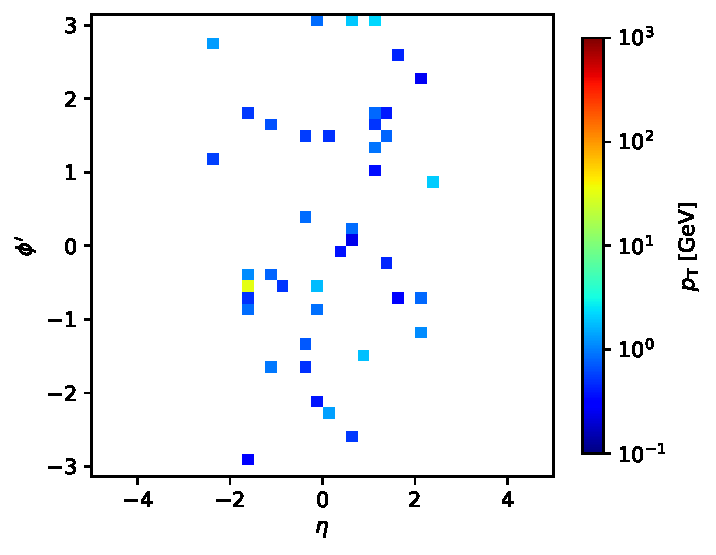
\includegraphics[width=0.45\textwidth]{event_image_VBF-track.pdf}
            } \\
            \subfloat[GGF: Photon]{
                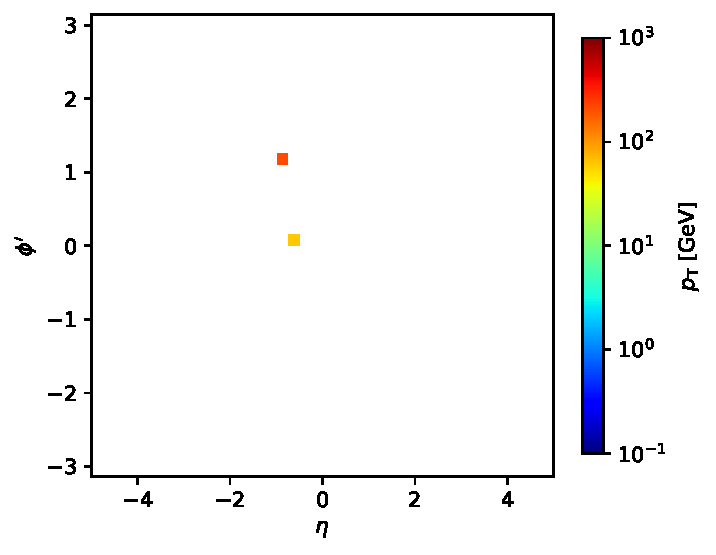
\includegraphics[width=0.45\textwidth]{event_image_GGF-photon.pdf}
            }
            \subfloat[VBF: Photon]{
                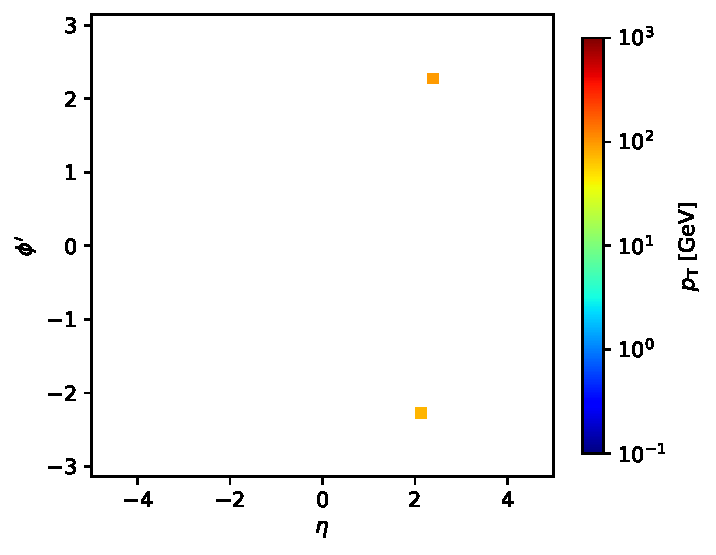
\includegraphics[width=0.45\textwidth]{event_image_VBF-photon.pdf}
            }
            \caption{Event images for GGF and VBF production, separately shown for calorimeter towers, tracks, and photons.}
            \label{fig:GGF_VEF_event_image}
        \end{figure}
    % subsection event_image (end)
    \subsection{Mixed datasets}% (fold)
    \label{sub:mixed_datasets}
        Based on figure~\ref{fig:mjj_deta_distribution}, we set selection cuts of $m_{jj} > 300$ GeV and $\Delta\eta_{jj} > 3.1$. We consider three cases: applying each cut individually and applying both cuts simultaneously. These cuts define the signal region (SR), which is VBF-like, and the background region (BR), which is GGF-like. Table~\ref{tab:GGF_VBF_Higgs_cutflow_number_mixed_dataset} summarizes the cutflow results for different selection criteria.
        \begin{table}[htpb]
            \centering
            \caption{Number of passing events and passing rates for GGF and VBF Higgs production under different selection cuts.}
            \label{tab:GGF_VBF_Higgs_cutflow_number_mixed_dataset}
            \begin{tabular}{l|rr|rr}
                Cut                                & GGF    & pass rate & VBF    & pass rate \\ \hline
                Total                              & 100000 & 1.00      & 100000 & 1.00      \\
                $n_{\gamma}$ cut                   & 9302   & 0.09      & 42860  & 0.43      \\
                $n_j$ cut                          & 9302   & 0.09      & 42860  & 0.43      \\
                $m_{\gamma\gamma}$ cut             & 8864   & 0.09      & 40694  & 0.41      \\ \hline
                $m_{jj}$ cut: SR                   & 2695   & 0.03      & 29496  & 0.29      \\
                $m_{jj}$ cut: BR                   & 6169   & 0.06      & 11198  & 0.11      \\ \hline
                $\Delta\eta_{jj}$ cut: SR          & 2317   & 0.02      & 28160  & 0.28      \\
                $\Delta\eta_{jj}$ cut: BR          & 6547   & 0.07      & 12534  & 0.13      \\ \hline
                $m_{jj}, \Delta\eta_{jj}$ cuts: SR & 1832   & 0.02      & 26446  & 0.26      \\
                $m_{jj}, \Delta\eta_{jj}$ cuts: BR & 5684   & 0.06      & 9484   & 0.09     
            \end{tabular}
        \end{table}

        The total cross-section for VBF production is $\sigma_{\text{VBF}} = 4.278$ pb$^{-1}$ at NNLO and for GGF production is $\sigma_{\text{GGF}} = 54.67$ pb$^{-1}$ at N3LO, as referenced in \href{https://twiki.cern.ch/twiki/bin/view/LHCPhysics/CERNYellowReportPageAt14TeV}{this link}. The branching ratio for the di-photon decay channel is $\Gamma\left( h \to \gamma\gamma \right) = 2.270 \times 10^{-3}$, as given in \href{https://twiki.cern.ch/twiki/bin/view/LHCPhysics/CERNYellowReportPageBR}{this link}.

        Assuming the luminosity of $\mathcal{L} = \text{300 fb}^{-1}$, we can estimate the number of events belonging to the SR and BR. These results are summarized in table~\ref{tab:number_of_event_in_mixed_dataset}
        \begin{table}[htpb]
            \centering
            \caption{The number of events of mixed datasets under different selection cuts.}
            \label{tab:number_of_event_in_mixed_dataset}
            \subfloat[$m_{jj} > 300$ GeV]{
                \begin{tabular}{c|cc}
                       & GGF & VBF \\ \hline
                    BR & 2297 & 326 \\
                    SR & 1003 & 859
                \end{tabular}
            }
            \subfloat[$\Delta\eta_{jj} > 3.1$]{
                \begin{tabular}{c|cc}
                       & GGF & VBF \\ \hline
                    BR & 2437 & 365 \\
                    SR & 863  & 820
                \end{tabular}
            } \\
            \subfloat[$m_{jj} > 300$ GeV, \newline $\Delta\eta_{jj} > 3.1$]{
                \begin{tabular}{c|cc}
                       & GGF & VBF \\ \hline
                    BR & 2116 & 276 \\
                    SR & 682  & 770
                \end{tabular}
            }
        \end{table}
    % subsection mixed_datasets (end)
    \subsection{Training CNN}% (fold)
    \label{sub:training_cnn}
        The total sample sizes are mentioned in section~\ref{sub:mixed_datasets}. We allocate 80\% of the data for training and 20\% for validation. The testing set consists of the SR's 10,000 VBF and 10,000 GGF events.

        The convolutional neural network (CNN) model structure is summarized in figure~\ref{fig:cnn_model_structure}. The internal node uses the rectified linear unit (ReLU) as the activation function. The loss function is the binary cross-entropy. The \verb|Adam| optimizer minimizes the loss value. The learning rate is $10^{-4}$, and the batch size is 512. We employ the early stopping technique to prevent over-training issues with a patience of 10.
        \begin{figure}[htpb]
            \centering
            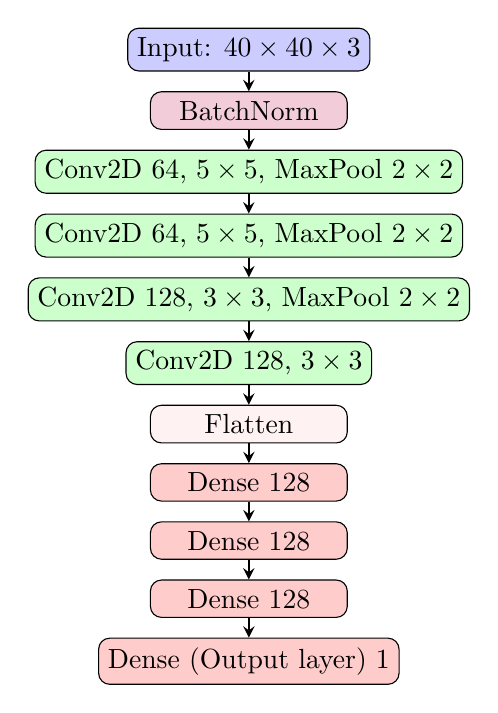
\begin{tikzpicture}[
                layer/.style={draw, rounded corners, minimum width=2.5cm, text centered},
                arrow/.style={-stealth, thick},
                node distance=0.25cm,
            ]
            % Input layer
            \node (input) [layer, fill=blue!20,] {Input: $40 \times 40 \times 3$};

            % Jet 1 layers
            \node (bn1) [below=of input, layer, fill=purple!20] {BatchNorm};


            % Conv1_1 layer positioned between bn1 and bn2
            \node (conv1_1) [below=0.25cm of bn1, layer, fill=green!20] {Conv2D 64, $5 \times 5$, MaxPool $2 \times 2$};

            % Other Conv layers
            \node (conv2_1) [below=of conv1_1, layer, fill=green!20] {Conv2D 64, $5 \times 5$, MaxPool $2 \times 2$};
            \node (conv3_1) [below=of conv2_1, layer, fill=green!20] {Conv2D 128, $3 \times 3$, MaxPool $2 \times 2$};
            \node (conv4_1) [below=of conv3_1, layer, fill=green!20] {Conv2D 128, $3 \times 3$};

            % Dense layers
            \node (flatten1) [below=of conv4_1, layer, fill=pink!20] {Flatten};
            \node (dense1_1) [below=of flatten1, layer, fill=red!20] {Dense 128};
            \node (dense2_1) [below=of dense1_1, layer, fill=red!20] {Dense 128};
            \node (dense3_1) [below=of dense2_1, layer, fill=red!20] {Dense 128};
            \node (output1) [below=of dense3_1, layer, fill=red!20] {Dense (Output layer) 1};


            % Arrows for BN
            \draw [arrow] (input) -- (bn1);
            \draw [arrow] (bn1) -- (conv1_1);
            \draw [arrow] (conv1_1) -- (conv2_1);
            \draw [arrow] (conv2_1) -- (conv3_1);
            \draw [arrow] (conv3_1) -- (conv4_1);
            \draw [arrow] (conv4_1) -- (flatten1);
            \draw [arrow] (flatten1) -- (dense1_1);
            \draw [arrow] (dense1_1) -- (dense2_1);
            \draw [arrow] (dense2_1) -- (dense3_1);
            \draw [arrow] (dense3_1) -- (output1);

            \end{tikzpicture}
            \caption{The architecture of the CNN model with key hyperparameters.}
            \label{fig:cnn_model_structure}
        \end{figure}

        The training results are summarized in table~\ref{tab:CWoLa_CNN_training_results}. The performance of the $\Delta\eta_{jj}$ cuts is better than the $m_{jj}$ cut. Moreover, when both cuts are applied together, the performance is slightly worse than when applying either cut individually.
        \begin{table}[htpb]
            \centering
            \caption{The CNN training results. The ACC and AUC are evaluated based on 10 training. The selection cuts of $m_{jj} > \text{300 GeV}$ and $\Delta\eta_{jj} > 3.1$ are applied.}
            \label{tab:CWoLa_CNN_training_results}
            \begin{tabular}{l|cc|cc}
                                          & \multicolumn{2}{c|}{$M_1 / M_2$}      & \multicolumn{2}{c}{$S / B$}           \\ \hline
                Cut                       & ACC               & AUC               & ACC               & AUC               \\ \hline
                $m_{jj}$                  & $0.712 \pm 0.023$ & $0.741 \pm 0.041$ & $0.576 \pm 0.010$ & $0.596 \pm 0.014$ \\
                $\Delta\eta_{jj}$         & $0.828 \pm 0.043$ & $0.889 \pm 0.050$ & $0.604 \pm 0.014$ & $0.630 \pm 0.015$ \\
                $m_{jj}, \Delta\eta_{jj}$ & $0.753 \pm 0.022$ & $0.792 \pm 0.035$ & $0.573 \pm 0.007$ & $0.596 \pm 0.008$
            \end{tabular}
        \end{table}
    % subsection training_cnn (end)
    \subsection{More events}% (fold)
    \label{sub:more_events}
        This section assumes the luminosity of $\mathcal{L} = \text{3000 fb}^{-1}$. The number of events belonging to the SR and BR are summarized in table~\ref{tab:number_of_event_in_mixed_dataset_3000}.
        \begin{table}[htpb]
            \centering
            \caption{The number of events of mixed datasets under different selection cuts.}
            \label{tab:number_of_event_in_mixed_dataset_3000}
            \subfloat[$m_{jj} > 300$ GeV]{
                \begin{tabular}{c|cc}
                       & GGF & VBF \\ \hline
                    BR & 22967 & 3262 \\
                    SR & 10034 & 8593
                \end{tabular}
            }
            \subfloat[$\Delta\eta_{jj} > 3.1$]{
                \begin{tabular}{c|cc}
                       & GGF & VBF \\ \hline
                    BR & 24375 & 3652 \\
                    SR & 8626  & 8204
                \end{tabular}
            } \\
            \subfloat[$m_{jj} > 300$ GeV, \newline $\Delta\eta_{jj} > 3.1$]{
                \begin{tabular}{c|cc}
                       & GGF & VBF \\ \hline
                    BR & 21162 & 2763 \\
                    SR & 6821  & 7705
                \end{tabular}
            }
        \end{table}

        The training results are summarized in table~\ref{tab:CWoLa_CNN_training_results_3000}. All datasets' performance is better than the results in table~\ref{tab:CWoLa_CNN_training_results}. The $\Delta\eta_{jj}$ cut performs better than the $m_{jj}$ cut. Moreover, when both cuts are applied together, the performance is slightly worse than the $\Delta\eta_{jj}$ cut but better than $m_{jj}$. These results are similar to the previous one. 
        \begin{table}[htpb]
            \centering
            \caption{The CNN training results. The ACC and AUC are evaluated based on 10 training. The selection cuts of $m_{jj} > \text{300 GeV}$ and $\Delta\eta_{jj} > 3.1$ are applied.}
            \label{tab:CWoLa_CNN_training_results_3000}
            \begin{tabular}{l|cc|cc}
                                          & \multicolumn{2}{c|}{$M_1 / M_2$}      & \multicolumn{2}{c}{$S / B$}           \\ \hline
                Cut                       & ACC               & AUC               & ACC               & AUC               \\ \hline
                $m_{jj}$                  & $0.907 \pm 0.002$ & $0.969 \pm 0.002$ & $0.598 \pm 0.008$ & $0.625 \pm 0.009$ \\
                $\Delta\eta_{jj}$         & $0.931 \pm 0.004$ & $0.979 \pm 0.002$ & $0.615 \pm 0.005$ & $0.648 \pm 0.006$ \\
                $m_{jj}, \Delta\eta_{jj}$ & $0.929 \pm 0.003$ & $0.978 \pm 0.002$ & $0.608 \pm 0.004$ & $0.638 \pm 0.005$
            \end{tabular}
        \end{table}
    % subsection more_events (end)
% section sample_preparation (end)
\bibliographystyle{ieeetr}
\bibliography{reference}

\end{document}
